%! TEX root = main.tex

\subsection{Darcy-Weisbach bottom friction}

Equation \ref{eq:swe} lumps viscosity effects into bottom friction forces ($F_x$ and $F_y$), which can be calculated with either the Manning equation or Darcy-Weisbach equation.
Manning equation and Darcy-Weisbach equation were originally developed for closed-pipe and open-channel flows. 
Practitioners also apply them to overland flow as they deem overland flow as infinite-width open-channel flow. (\cite{bellos_friction_2018})
Well-justified bottom friction models for overland flows, to the best of our knowledge, do not exist yet.

We implemented Darcy-Weisbach models for friction forces in our code. We will discuss why we prefer Darcy-Weisbach models over the Manning equation later in section \ref{sec:discussion}. The Darcy-Weisbach equation is:

\begin{equation}
    \begin{bmatrix} F_x \\ F_y \end{bmatrix}
    =
    \gamma(\boldsymbol{q})\begin{bmatrix} hu \\ hv \end{bmatrix}
    =
    \frac{f}{8h^2}\sqrt{(hu)^2+(hv)^2}\begin{bmatrix} hu \\ hv \end{bmatrix}
\end{equation}
$f$ is the Darcy-Weisbach coefficient.
Different Darcy-Weisbach models rely on different empirical equations to calculate the Darcy-Weisbach coefficient.

Our code support two different models (\cite{cheng_formulas_2008, bellos_friction_2018}) to calculate the Darcy-Weisbach coefficient. Figure \ref{fig:darcy-weisbach-models} shows the friction coefficients calculated using the two models under different surface roughness.

\begin{figure}
    \centering
    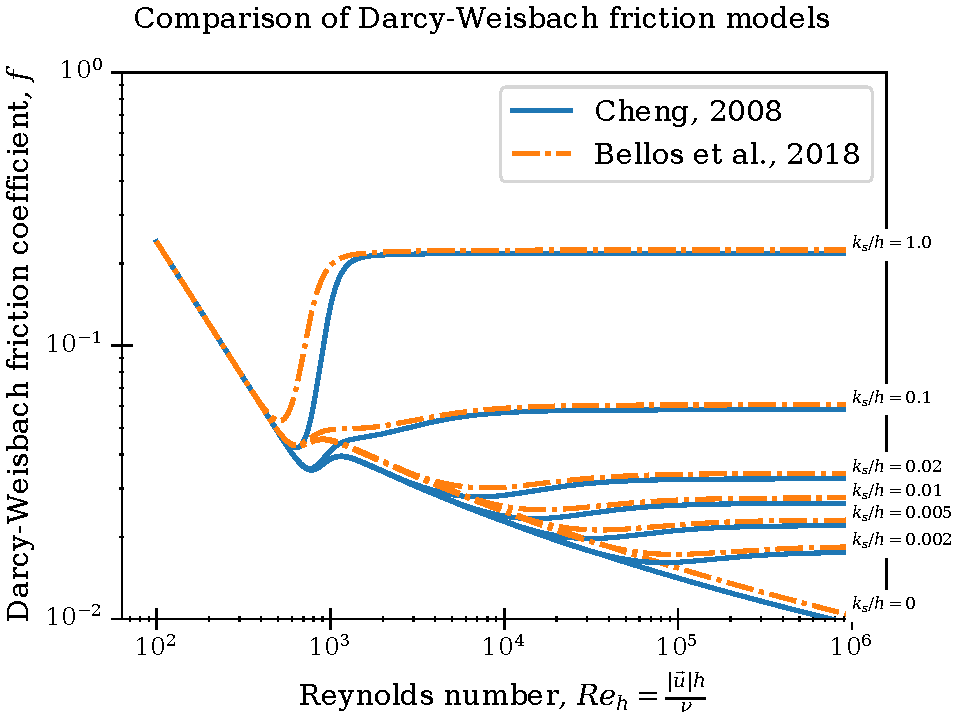
\includegraphics[width=0.9\linewidth]{darcy-weisbach-models}
    \caption{%
        Comparing the friction coefficients from the models in \cite{cheng_formulas_2008} and \cite{bellos_friction_2018} with different surface roughness $k_s$.
    }\label{fig:darcy-weisbach-models}
\end{figure}

\subsubsection{\cite{cheng_formulas_2008}}

Cheng proposed the following formula, which covers flow regimes from laminar to fully-rough turbulent flow:
\begin{equation}
    \begin{split}
        &\begin{multlined}
            f =
            \left( \frac{24}{Re_h} \right)^\alpha
            \times
            \left( 1.8\log_{10}\frac{Re_h}{2.1} \right)^{-2\left(1-\alpha\right)\beta}
            \\
            \times
            \left( 2\log_{10}\frac{11.8h}{k_s} \right)^{-2\left(1-\alpha\right)\left(1-\beta\right)}
        \end{multlined}\\
        &\alpha=\left[1+\left(\frac{Re_h}{850}\right)^9\right]^{-1}
        \text{, }
        \beta=\left[1+\left(\frac{Re_h k_s}{160h}\right)^2\right]^{-1}
    \end{split}
\end{equation}
$Re_h\equiv\frac{h\sqrt{u^2+v^2}}{\nu}$ is the Reynolds number defined with flow depth $h$ and kinematic viscosity $\nu$.
$k_s$ denotes the characteristic length of surface roughness. 

\subsubsection{\cite{bellos_friction_2018}}

Bellos, Nalbantis, and Tsakiris proposed an alternative formula for flood flow (we re-arranged it for clarity):
\begin{equation}
    \begin{split}
        &\begin{multlined}
            f =
            \left( \frac{24}{Re_h} \right)^\alpha
            \times
            \left( \frac{\sqrt{8}}{C_sRe_h}e^{1+W(\frac{\kappa}{e}C_sRe_h)} \right)^{2\left(1-\alpha\right)\beta}
            \\
            \times
            \left( \sqrt{8}\kappa\ln^{-1}(\frac{C_r}{e}\frac{h}{k_s}) \right)^{2\left(1-\alpha\right)\left(1-\beta\right)}
        \end{multlined} \\
        &\alpha=\left[1+\left(\frac{Re_h}{678}\right)^{8.4}\right]^{-1}
        \text{, }
        \beta=\left[1+\left(\frac{Re_h k_s}{150h}\right)^{1.8}\right]^{-1}.
    \end{split}
\end{equation}
$e$ and $\kappa\approx 0.4187$ denote Euler's number and the von Karman constant, respectively.
$C_s=8.94$ and $C_r=33.2$ are constants determined through fitting closed-pipe experimental data.
$W$ is an approximation to the Lambert W function: 
\begin{equation}
    \begin{multlined}
        W(x)
        =
        \ln(x)
        -
        \ln(\ln(x))
        +
        \frac{\ln(\ln(x))}{\ln(x)}
        \\
        +
        \frac{\ln^2(\ln(x))-2\ln(\ln(x))}{2\ln^2(x)}
    \end{multlined}
\end{equation}
This approximation has relative errors smaller than $0.1\%$ in the regime of smooth turbulent flow ($700 < Re_h < 25{,}000$).
Note this friction model, though designed for flood flow, is still based on 1D open-channel flow models and experimental data.
